% move all configuration stuff into include file so we can focus on the content
\documentclass[aspectratio=169,hyperref={pdfpagelabels=false,colorlinks=true,linkcolor=white,urlcolor=blue},t]{beamer}

%%%%%%%%%%%%%%%%%%%%%%%%%%%%%%%%%%%%%%%%%%%%%%%%%%%%%%%%%%%%%%%%%%%%%%%%%%%%%%%%%%
%%%%%%%%%%%%%%%%%%%%%%%%%%%%%%%%%%%%%%%%%%%%%%%%%%%%%%%%%%%%%%%%%%%%%%%%%%%%%%%%%%
% packages
\usepackage{pict2e}
\usepackage{epic}
\usepackage{amsmath,amsfonts,amssymb}
\usepackage{units}
\usepackage{fancybox}
\usepackage[absolute,overlay]{textpos} 
\usepackage{media9} % avi2flv: "C:\Program Files\ffmpeg\bin\ffmpeg.exe" -i TuneFreqFilterbank.avi -b 600k -s 441x324 -r 15 -acodec copy TuneFreqFilterbank.flv
\usepackage{animate}
\usepackage{gensymb}
\usepackage{multirow}
\usepackage{silence}
\usepackage{tikz}
\usepackage[backend=bibtex,style=ieee]{biblatex}
\AtEveryCitekey{\iffootnote{\tiny}{}}
\addbibresource{include/references}

%%%%%%%%%%%%%%%%%%%%%%%%%%%%%%%%%%%%%%%%%%%%%%%%%%%%%%%%%%%%%%%%%%%%%%%%%%%%%%%%%%
%%%%%%%%%%%%%%%%%%%%%%%%%%%%%%%%%%%%%%%%%%%%%%%%%%%%%%%%%%%%%%%%%%%%%%%%%%%%%%%%%%
% relative paths
\graphicspath{{graph/}}


%%%%%%%%%%%%%%%%%%%%%%%%%%%%%%%%%%%%%%%%%%%%%%%%%%%%%%%%%%%%%%%%%%%%%%%%%%%%%%%%%%
%%%%%%%%%%%%%%%%%%%%%%%%%%%%%%%%%%%%%%%%%%%%%%%%%%%%%%%%%%%%%%%%%%%%%%%%%%%%%%%%%%
% units
\setlength{\unitlength}{1mm}

%%%%%%%%%%%%%%%%%%%%%%%%%%%%%%%%%%%%%%%%%%%%%%%%%%%%%%%%%%%%%%%%%%%%%%%%%%%%%%%%%%
%%%%%%%%%%%%%%%%%%%%%%%%%%%%%%%%%%%%%%%%%%%%%%%%%%%%%%%%%%%%%%%%%%%%%%%%%%%%%%%%%%
% theme & layout
\usetheme{Frankfurt}
\beamertemplatenavigationsymbolsempty
%\setbeamertemplate{frametitle}[smoothbars theme]
\setbeamertemplate{frametitle}
{
    \begin{beamercolorbox}[ht=1.8em,wd=\paperwidth]{frametitle}
        \vspace{-.1em}%
        \hspace{.2em}{\strut\insertframetitle\strut}
        
        \hspace{.2em}\small\strut\insertframesubtitle\strut
        %\hfill
        %\includegraphics[height=.8cm,keepaspectratio]{CenterMusicTechnology-solid-2lines-white-CoAtag}
        
    \end{beamercolorbox}
    \begin{textblock*}{100mm}(11.6cm,.7cm)
        \includegraphics[height=.8cm,keepaspectratio]{Logo_GTCMT_black}
    \end{textblock*}
}
\setbeamertemplate{footline}[frame number]

% set this to ensure bulletpoints without subsections
\usepackage{remreset}
\makeatletter
\@removefromreset{subsection}{section}
\makeatother
\setcounter{subsection}{1}

%---------------------------------------------------------------------------------
% appearance
\setbeamercolor{structure}{fg=gtgold}
\setbeamercovered{transparent} %invisible
\setbeamercolor{bibliography entry author}{fg=black}
\setbeamercolor*{bibliography entry title}{fg=black}
\setbeamercolor*{bibliography entry note}{fg=black}
\setbeamercolor{frametitle}{fg=black}
\setbeamercolor{title}{fg=black}

%\usepackage{pgfpages}
%\setbeameroption{show notes}
%\setbeameroption{show notes on second screen=right}
%---------------------------------------------------------------------------------
% fontsize
\let\Tiny=\tiny

%%%%%%%%%%%%%%%%%%%%%%%%%%%%%%%%%%%%%%%%%%%%%%%%%%%%%%%%%%%%%%%%%%%%%%%%%%%%%%%%%%
%%%%%%%%%%%%%%%%%%%%%%%%%%%%%%%%%%%%%%%%%%%%%%%%%%%%%%%%%%%%%%%%%%%%%%%%%%%%%%%%%%
% warnings
\pdfsuppresswarningpagegroup=1
\WarningFilter{biblatex}{Patching footnotes failed}
\WarningFilter{latexfont}{Font shape}
\WarningFilter{latexfont}{Some font shapes}
\WarningFilter{gensymb}{Not defining}


%%%%%%%%%%%%%%%%%%%%%%%%%%%%%%%%%%%%%%%%%%%%%%%%%%%%%%%%%%%%%%%%%%%%%%%%%%%%%%%%%%
%%%%%%%%%%%%%%%%%%%%%%%%%%%%%%%%%%%%%%%%%%%%%%%%%%%%%%%%%%%%%%%%%%%%%%%%%%%%%%%%%%
% theme & layout
\usetheme{Frankfurt}
\useinnertheme{rectangles}


%%%%%%%%%%%%%%%%%%%%%%%%%%%%%%%%%%%%%%%%%%%%%%%%%%%%%%%%%%%%%%%%%%%%%%%%%%%%%%%%%%
\setbeamertemplate{frametitle}[default][colsep=-4bp,rounded=false,shadow=false]
\setbeamertemplate{frametitle}
{%
    \nointerlineskip%
    %\vskip-0.5ex
    \begin{beamercolorbox}[wd=\paperwidth,ht=3.5ex,dp=0.6ex]{frametitle}
        \hspace*{1.3ex}\insertframetitle%
        
        \hspace*{1.3ex}\small\insertframesubtitle%
    \end{beamercolorbox}%
    \begin{textblock*}{100mm}(11.6cm,.57cm)
        
\includegraphics[height=.8cm,keepaspectratio]{graph/Logo_GTCMT_white}
    \end{textblock*}
}


%%%%%%%%%%%%%%%%%%%%%%%%%%%%%%%%%%%%%%%%%%%%%%%%%%%%%%%%%%%%%%%%%%%%%%%%%%%%%%%%%%
\setbeamertemplate{title page}[default][colsep=-4bp,rounded=false,shadow=false]
\setbeamertemplate{title page}
{
    \begin{textblock*}{100mm}(15cm,.51cm)
            \href{https://github.com/alexanderlerch/ACA-Slides/blob/2nd_edition/\jobname.pdf}{\includegraphics[height=.5cm,keepaspectratio]{graph/Logo_github}}\hspace*{2ex}
    \end{textblock*}
    \vskip-10ex
    \begin{beamercolorbox}[wd=\paperwidth,ht=.7\paperheight,dp=0.6ex]{frametitle} %35ex
        %\begin{flushright}
            %\href{http://www.gtcmt.gatech.edu}{\includegraphics[height=.8cm,keepaspectratio]{graph/Logo_GTCMT_black}}\hspace*{2ex}
        %\end{flushright}
        
        \hspace*{1.8ex}\LARGE\inserttitle%
        
        \vspace*{.5ex}
        
        \hspace*{1.3ex}\small\insertsubtitle%
        
        \vspace*{.5ex}
    \end{beamercolorbox}%
    \nointerlineskip%
    \begin{beamercolorbox}[wd=\paperwidth,ht=.4\paperheight,dp=0.6ex]{page number in head/foot}
        %\vspace*{-.5ex}
        \hspace*{1.7ex}\small\insertauthor%
        
        %\hspace*{1.7ex}\small }%
        
        \vspace*{10ex}
        
        \begin{flushright}
            \href{http://www.gtcmt.gatech.edu}{\includegraphics[height=.8cm,keepaspectratio]{graph/Logo_GTCMT_black}}\hspace*{2ex}
        \end{flushright}
    \end{beamercolorbox}%
}


%%%%%%%%%%%%%%%%%%%%%%%%%%%%%%%%%%%%%%%%%%%%%%%%%%%%%%%%%%%%%%%%%%%%%%%%%%%%%%%%%%
%\makeatother
\setbeamertemplate{footline}
{
  \leavevmode%
  \hbox{%
  \begin{beamercolorbox}[wd=.5\paperwidth,ht=2.25ex,dp=1ex,left,leftskip=1ex]{page number in head/foot}%
    \insertsubtitle
  \end{beamercolorbox}%
  \begin{beamercolorbox}[wd=.5\paperwidth,ht=2.25ex,dp=1ex,right,rightskip=1ex]{page number in head/foot}%
    \hfill
    \insertframenumber{} / \inserttotalframenumber
  \end{beamercolorbox}}%
  \vskip0pt%
}
%\makeatletter


%%%%%%%%%%%%%%%%%%%%%%%%%%%%%%%%%%%%%%%%%%%%%%%%%%%%%%%%%%%%%%%%%%%%%%%%%%%%%%%%%%
\beamertemplatenavigationsymbolsempty
\setbeamertemplate{navigation symbols}{}
\setbeamertemplate{blocks}[default]%[rounded=false,shadow=false]
\setbeamertemplate{itemize item}[square]
\setbeamertemplate{itemize subitem}[circle]
\setbeamertemplate{itemize subsubitem}[triangle]
\setbeamertemplate{enumerate item}[square]
\setbeamertemplate{enumerate subitem}[circle]
\setbeamertemplate{enumerate subsubitem}[circle]


%%%%%%%%%%%%%%%%%%%%%%%%%%%%%%%%%%%%%%%%%%%%%%%%%%%%%%%%%%%%%%%%%%%%%%%%%%%%%%%%%%
% colors
\setbeamercolor{structure}{fg=darkgray}
\setbeamercovered{transparent} %invisible
\setbeamercolor{bibliography entry author}{fg=black}
\setbeamercolor*{bibliography entry title}{fg=black}
\setbeamercolor*{bibliography entry note}{fg=black}
\setbeamercolor{frametitle}{fg=black}
\setbeamercolor{title}{fg=white}
\setbeamercolor{subtitle}{fg=white}
\setbeamercolor{frametitle}{fg=white}
\setbeamercolor{framesubtitle}{fg=white}
\setbeamercolor{mini frame}{fg=white, bg=black}
\setbeamercolor{section in head/foot}{fg=white, bg=darkgray}
\setbeamercolor{page number in head/foot}{fg=black, bg=lightblue}
\setbeamercolor{item projected}{fg=white, bg=black}

%---------------------------------------------------------------------------------
%%%%%%%%%%%%%%%%%%%%%%%%%%%%%%%%%%%%%%%%%%%%%%%%%%%%%%%%%%%%%%%%%%%%%%%%%%%%%%%%%%
%%%%%%%%%%%%%%%%%%%%%%%%%%%%%%%%%%%%%%%%%%%%%%%%%%%%%%%%%%%%%%%%%%%%%%%%%%%%%%%%%%
% title information
\title[]{Introduction to \textbf{Audio Content Analysis}}   
\author[alexander lerch]{alexander lerch} 
%\institute{~}
%\date[Alexander Lerch]{}
%\titlegraphic{\vspace{-16mm}\includegraphics[width=\textwidth,height=3cm]{title}}

%%%%%%%%%%%%%%%%%%%%%%%%%%%%%%%%%%%%%%%%%%%%%%%%%%%%%%%%%%%%%%%%%%%%%%%%%%%%%%%%%%
%%%%%%%%%%%%%%%%%%%%%%%%%%%%%%%%%%%%%%%%%%%%%%%%%%%%%%%%%%%%%%%%%%%%%%%%%%%%%%%%%%
% colors
\definecolor{gtgold}{HTML}{E0AA0F} %{rgb}{0.88,0.66,1,0.06} [234, 170, 0]/256
\definecolor{darkgray}{rgb}{.1, .1, .25}
\definecolor{lightblue}{rgb}{.1, 0.75, 1}
\definecolor{highlight}{rgb}{0, 0, 1} %_less!40

%%%%%%%%%%%%%%%%%%%%%%%%%%%%%%%%%%%%%%%%%%%%%%%%%%%%%%%%%%%%%%%%%%%%%%%%%%%%%%%%%%
%%%%%%%%%%%%%%%%%%%%%%%%%%%%%%%%%%%%%%%%%%%%%%%%%%%%%%%%%%%%%%%%%%%%%%%%%%%%%%%%%%
% relative paths
\graphicspath{{../ACA-Plots/graph/}}


%%%%%%%%%%%%%%%%%%%%%%%%%%%%%%%%%%%%%%%%%%%%%%%%%%%%%%%%%%%%%%%%%%%%%%%%%%%%%%%%%%
%%%%%%%%%%%%%%%%%%%%%%%%%%%%%%%%%%%%%%%%%%%%%%%%%%%%%%%%%%%%%%%%%%%%%%%%%%%%%%%%%%
% units
\setlength{\unitlength}{1mm}

%%%%%%%%%%%%%%%%%%%%%%%%%%%%%%%%%%%%%%%%%%%%%%%%%%%%%%%%%%%%%%%%%%%%%%%%%%%%%%%%%%
%%%%%%%%%%%%%%%%%%%%%%%%%%%%%%%%%%%%%%%%%%%%%%%%%%%%%%%%%%%%%%%%%%%%%%%%%%%%%%%%%%
% math
\DeclareMathOperator*{\argmax}{argmax}
\DeclareMathOperator*{\argmin}{argmin}
\DeclareMathOperator*{\atan}{atan}
\DeclareMathOperator*{\arcsinh}{arcsinh}
\DeclareMathOperator*{\sign}{sign}
\DeclareMathOperator*{\tcdf}{tcdf}
\DeclareMathOperator*{\si}{sinc}
\DeclareMathOperator*{\princarg}{princarg}
\DeclareMathOperator*{\arccosh}{arccosh}
\DeclareMathOperator*{\hwr}{HWR}
\DeclareMathOperator*{\flip}{flip}
\DeclareMathOperator*{\sinc}{sinc}
\DeclareMathOperator*{\floor}{floor}
\newcommand{\e}{{e}}
\newcommand{\jom}{\mathrm{j}\omega}
\newcommand{\jOm}{\mathrm{j}\Omega}
\newcommand   {\mat}[1]    		{\boldsymbol{\uppercase{#1}}}		%bold
\renewcommand {\vec}[1]    		{\boldsymbol{\lowercase{#1}}}		%bold

%%%%%%%%%%%%%%%%%%%%%%%%%%%%%%%%%%%%%%%%%%%%%%%%%%%%%%%%%%%%%%%%%%%%%%%%%%%%%%%%%%
%%%%%%%%%%%%%%%%%%%%%%%%%%%%%%%%%%%%%%%%%%%%%%%%%%%%%%%%%%%%%%%%%%%%%%%%%%%%%%%%%%
% media9
\newcommand{\includeaudio}[1]{
\href{run:audio/#1.mp3}{
\includegraphics[width=5mm, height=5mm]{graph/SpeakerIcon}}}

\newcommand{\includeanimation}[4]{{\begin{center}
                        \animategraphics[autoplay,loop,scale=.7]{#4}{animation/#1-}{#2}{#3}        
                        \end{center}
                        \addreference{matlab source: \href{https://github.com/alexanderlerch/ACA-Plots/blob/master/matlab/animate#1.m}{matlab/animate#1.m}}}
                        \inserticon{video}}
                        
%%%%%%%%%%%%%%%%%%%%%%%%%%%%%%%%%%%%%%%%%%%%%%%%%%%%%%%%%%%%%%%%%%%%%%%%%%%%%%%%%%
%%%%%%%%%%%%%%%%%%%%%%%%%%%%%%%%%%%%%%%%%%%%%%%%%%%%%%%%%%%%%%%%%%%%%%%%%%%%%%%%%%
% other commands
\newcommand{\question}[1]{%\vspace{-4mm}
                          \setbeamercovered{invisible}
                          \begin{columns}[T]
                            \column{.9\textwidth}
                                \textbf{#1}
                            \column{.1\textwidth}
                                \vspace{-8mm}
                                \begin{flushright}
                                     
\includegraphics[width=.9\columnwidth]{graph/question_mark}
                                \end{flushright}
                                \vspace{6mm}
                          \end{columns}\pause\vspace{-12mm}}

\newcommand{\toremember}[1]{
                        \inserticon{lightbulb}
                        }

\newcommand{\matlabexercise}[1]{%\vspace{-4mm}
                          \setbeamercovered{invisible}
                          \begin{columns}[T]
                            \column{.8\textwidth}
                                \textbf{matlab exercise}: #1
                            \column{.2\textwidth}
                                \begin{flushright}
                                     \includegraphics[scale=.5]{graph/logo_matlab}
                                \end{flushright}
                                %\vspace{6mm}
                          \end{columns}}

\newcommand{\addreference}[1]{  
                  
                    \begin{textblock*}{\baselineskip }(.98\paperwidth,.5\textheight) %(1.15\textwidth,.4\textheight)
                         \begin{minipage}[b][.5\paperheight][b]{1cm}%
                            \vfill%
                             \rotatebox{90}{\tiny {#1}}
                        \end{minipage}
                   \end{textblock*}
                    }
                    
\newcommand{\figwithmatlab}[1]{
                    \begin{figure}
                        \centering
                        \includegraphics[scale=.7]{#1}
                        %\label{fig:#1}
                    \end{figure}
                    
                    \addreference{matlab source: \href{https://github.com/alexanderlerch/ACA-Plots/blob/main/matlab/plot#1.m}{plot#1.m}}}
\newcommand{\figwithref}[2]{
                    \begin{figure}
                        \centering
                        \includegraphics[scale=.7]{#1}
                        \label{fig:#1}
                    \end{figure}
                    
                    \addreference{#2}}  
                                    
\newcommand{\inserticon}[1]{
                    \begin{textblock*}{100mm}(14.5cm,7.5cm)
                        \includegraphics[height=.8cm,keepaspectratio]{graph/#1}
                    \end{textblock*}}            

%%%%%%%%%%%%%%%%%%%%%%%%%%%%%%%%%%%%%%%%%%%%%%%%%%%%%%%%%%%%%%%%%%%%%%%%%%%%%%%%%%
%%%%%%%%%%%%%%%%%%%%%%%%%%%%%%%%%%%%%%%%%%%%%%%%%%%%%%%%%%%%%%%%%%%%%%%%%%%%%%%%%%
% counters
\newcounter{i}
\newcounter{j}
\newcounter{iXOffset}
\newcounter{iYOffset}
\newcounter{iXBlockSize}
\newcounter{iYBlockSize}
\newcounter{iYBlockSizeDiv2}
\newcounter{iXBlockSizeDiv2}
\newcounter{iDistance}




\subtitle{Module 1.0: Introduction to MIR/ACA}

%%%%%%%%%%%%%%%%%%%%%%%%%%%%%%%%%%%%%%%%%%%%%%%%%%%%%%%%%%%%%%%%%%%%%%%%%%%%
\begin{document}
    % generate title page
	{
\setbeamertemplate{headline}{} 
\setbeamertemplate{footline}{} 
\begin{frame}
    \titlepage
    %\vspace{-5mm}
\end{frame}
}
\addtocounter{framenumber}{-1}


    \section[overview]{lecture overview}
        \begin{frame}{introduction}{overview}
            \begin{block}{corresponding textbook section}
                    %\href{http://ieeexplore.ieee.org/xpl/articleDetails.jsp?tp=&arnumber=6331118&}{Chapter 1~---~Introduction}: pp.~1--6
                    Chapter~1
            \end{block}
            \vspace{5mm}

            \begin{itemize}
                \item   \textbf{lecture content}
                    \begin{itemize}
                        \item   audio content analysis
                        \item   typical applications
                        %\item   audio content
                        %\item   processing steps in a typical ACA system
                    \end{itemize}
                \bigskip
                \item<2->   \textbf{learning objectives}
                    \begin{itemize}
                        \item   list goals and applications in ACA
                        \item   understand the general development of the field
                        \item   differentiate various fields related to ACA
                        %\item   discuss typical forms of content in an audio signal
                        %\item   describe the typical signal flow in an ACA system
                    \end{itemize}
            \end{itemize}
            \inserticon{directions}
        \end{frame}
        
    \section[intro]{introduction}
        \begin{frame}{introduction}{content in audio signals}
             \begin{columns}
             \column{.4\textwidth}
                examples for audio signal content
                \begin{itemize}
                    \item   \textbf{speech}
                        \begin{itemize}
                            \item   text information
                            \item   speaker
                            \item   recording environment
                            \item   \dots
                        \end{itemize}
                    \item   \textbf{music}
                        \begin{itemize}
                            \item   melody
                            \item   harmony
                            \item   structure
                            \item   instruments
                            \item   mood
                            \item   genre
                            \item   \dots
                        \end{itemize}
                \end{itemize}
             \column{.6\textwidth}
                \figwithmatlab{Waveform}
                %\begin{figure}
                    %\includegraphics[scale=.4]{waveform}
                %\end{figure}
             \end{columns}
        \end{frame}
 
    \section[aca]{audio content analysis}
        \begin{frame}{introduction}{audio content analysis --- goals}
            \begin{block}{Audio Content Analysis}
                The field of Audio Content Analysis (ACA) aims at designing and applying algorithms for the \textbf{automatic extraction of content information from the raw (digital) audio signal}. 
                
                This enables content-driven and content-adaptive services which describe, categorize, sort, retrieve, segment, process, and visualize the signal and its content.                
            \end{block}
        \end{frame}
        
        \begin{frame}{introduction}{audio content analysis --- research fields}
            \vspace{-3mm}
            \begin{itemize}
                \item   \textbf{speech} analysis
                    \begin{itemize}
                        \item   speech recognition
                        \item   speech emotion recognition
                        \item   \ldots
                    \end{itemize}
                \smallskip
                \item<2->   \textbf{urban sound} analysis
                    \begin{itemize}
                        \item   noise pollution monitoring
                        \item   audio surveillance
                        \item   \ldots
                    \end{itemize}
                \smallskip
                \item<3->   \textbf{industrial sound} analysis
                    \begin{itemize}
                        \item   monitoring the state of mechanical devices (engines, etc.)
                        \item   monitoring the health of livestock
                        \item   \ldots
                    \end{itemize}
                \smallskip
                \item<4->   \only<5->{\textcolor{highlight}}{\textbf{musical audio} analysis}
                    \begin{itemize}
                        \item   music transcription
                        \item   music classification
                    \end{itemize}
            \end{itemize}
        \end{frame}
        
        \begin{frame}{introduction}{musical audio vs.\ other audio}
            \vspace{-3mm}
            \textbf{music} \ldots
            \begin{itemize}
                \item   is a \textbf{wide band} signal\\ unlike many other audio signals
                \item<2->   comprises both \textbf{tonal and noise} components\\ like most audio signals
                \item<3->   combines \textbf{multiple sound sources}\\ unlike speech, like urban sound
                \item<4->   is a \textbf{poly-timbral} mixture\\ unlike industrial sound
                \item<5->  sources are \textbf{harmonically related and synchronous}\\ unlike other multi-source signals
                \item<6->   has a highly structured language that is \textbf{abstract}\\ unlike speech
            \end{itemize}
        \end{frame}
        
        \begin{frame}{introduction}{audio content analysis --- related terms and areas}
            \begin{itemize}
                \item   \textbf{terminology}
                    \bigskip
                    \begin{itemize}
                        \item   \textit{Music Informatics}
                            \begin{itemize}
                                \item   overarching term for nearly everything with music and computers
                            \end{itemize}
                                
                        \smallskip
                        \item	\textit{Music Information Retrieval (MIR)}:
                            \begin{itemize}
                                \item   analysis and retrieval of music data 
                                \item   includes audio, symbolic, and other data
                                \item   might also cover other tasks (source separation, generation)
                            \end{itemize}
                                
                        \smallskip
                        \item	\textit{Machine Listening} \& \textit{Computer Audition}
                            \begin{itemize}
                                \item   focus on the recognition and understanding of music
                            \end{itemize}
                            
                        \smallskip
                        \item	\textit{Computational Auditory Scene Analysis (CASA)}
                            \begin{itemize}
                                \item   focus on human perception \& cognition, understanding of the auditory scene
                            \end{itemize}
                    \end{itemize}
           \end{itemize}
        \end{frame}
        \begin{frame}{introduction}{audio content analysis --- research field}
            \vspace{-7mm}
            \begin{columns}
            \column{.8\textwidth}
            \begin{itemize}
                \item<1->   \textbf{interdisciplinary}
                    \begin{itemize}
                        \item   digital signal processing
                        \item   machine learning / data mining
                        \item   musicology
                        \item   music psychology
                        \item   \ldots
                    \end{itemize}
                \smallskip
                \item<2->   ISMIR \textbf{community}
                            \begin{itemize}
                                \item   annual conferences 
                                \item   conference papers \& Transactions
                                \item   ISMIR-Community mailing list
                                \item   MIREX: MIR Evaluation eXchange
                            \end{itemize}
                \smallskip
                \item<3->   \textbf{related publication outlets} 
                    \begin{itemize}
                        \item   \textit{conferences}: ISMIR, ICASSP, ICME, SMC, DAFx, ACM~MM, \ldots
                        \item   \textit{journals}: TISMIR, TASLP, Computer Music, JNMR, JAES, \ldots
                    \end{itemize}
            \end{itemize}
            \column{.2\textwidth}
                \vspace{25mm}
                \begin{figure}
                    \includegraphics[height=.8cm,keepaspectratio]{graph/logo_ismir}
                \end{figure}
            \end{columns}
            \addreference{\href{http://www.ismir.net}{www.ismir.net}}
        \end{frame}
        \begin{frame}{introduction}{audio content analysis --- history}
            \begin{columns}
            \column{.5\textwidth}
            \begin{itemize}
                \item<1->   \textbf{historic}
                    \begin{itemize}
                        \item   mechanical devices
                    \end{itemize}
                \smallskip
                \item<2->   \textbf{expert systems}
                            \begin{itemize}
                                \item   rule-based approaches
                            \end{itemize}
                \smallskip
                \item<3->   data-driven \textbf{traditional ML systems }
                    \begin{itemize}
                        \item   feature design plus ML engine
                    \end{itemize}
                \smallskip
                \item<4->   \textbf{deep neural networks}
                    \begin{itemize}
                        \item   role of expert knowledge diminishes
                    \end{itemize}
            \end{itemize}
            \column{.5\textwidth}
                \begin{figure}
                    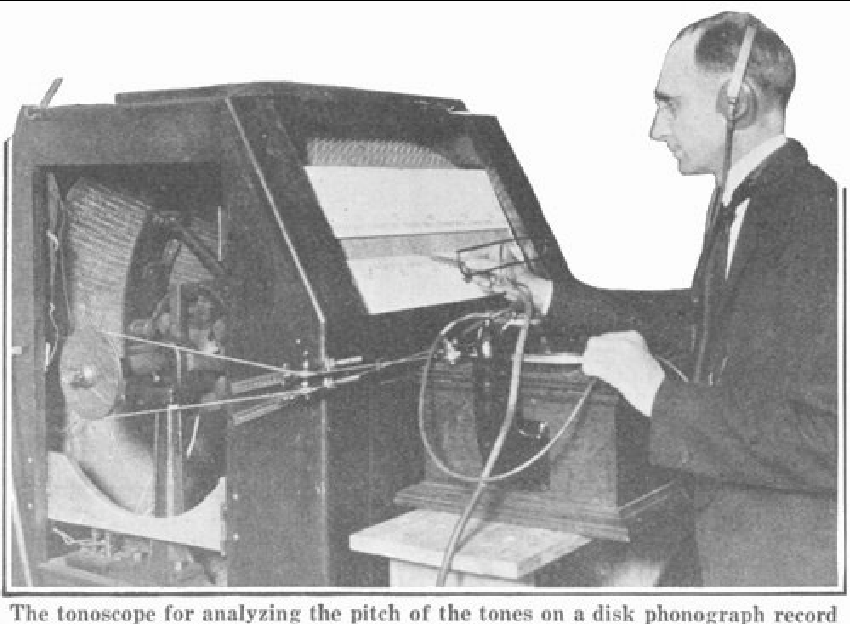
\includegraphics[width=\columnwidth]{graph/tonoscope}
                \end{figure}
            \end{columns}
        \end{frame}
        
    \section[apps]{applications}
        \begin{frame}{introduction}{applications}
            \begin{itemize}
                \item	\textbf{music browsing and music discovery} 
                    \begin{itemize}
                        \item   search \& retrieval, similarity, interfaces (e.g., QBH)
                    \end{itemize}
                \smallskip
                \item<2->	\textbf{music consumption} 
                    \begin{itemize}
                        \item   creative music listening
                    \end{itemize}
                \smallskip
                \item<3->	 \textbf{music production}
                    \begin{itemize}
                        \item   adaptive parametrization, enhancements of creative process
                    \end{itemize}
                \smallskip
                \item<4->	\textbf{music education}
                    \begin{itemize}
                        \item   musically intelligent software tutoring
                    \end{itemize}
                \smallskip
                \item<5->	\textbf{generative music}
                    \begin{itemize}
                        \item   interactive soundtracks (games, video)
                    \end{itemize}
            \end{itemize}
        \end{frame}
        \begin{frame}{introduction}{(commercial) application examples}
            \setbeamercovered{invisible} % uncover the graphics with the bullet points
            \begin{itemize}
                \item   \textbf{recommendation}, playlist generation
                    \begin{columns}
                        \column{.25\textwidth}
                        \column{.25\textwidth}
                            \href{https://www.spotify.com}{\includegraphics[scale=.1]{graph/logo_spotify}}
                        \column{.25\textwidth}
                            \href{https://www.last.fm}{\includegraphics[scale=.05]{graph/logo_lastfm}}
                        \column{.25\textwidth}
                            \href{https://www.pandora.com}{\includegraphics[scale=.03]{graph/logo_pandora}}
                    \end{columns}
                \bigskip
                \item<1->   \textbf{fingerprinting} 
                    \begin{columns}
                        \column{.25\textwidth}
                        \column{.25\textwidth}
                            \href{https://www.shazam.com}{\includegraphics[scale=.03]{graph/logo_shazam}}
                        \column{.25\textwidth}
                            \href{https://www.gracenote.com}{\includegraphics[scale=.05]{graph/logo_gracenote}}
                        \column{.25\textwidth}
                    \end{columns}
                \bigskip
                \item<1->   \textbf{score following} 
                   \begin{columns}
                        \column{.25\textwidth}
                        \column{.25\textwidth}
                            \href{http://www.rockprodigy.com}{\includegraphics[scale=.15]{graph/logo_rockprodigy}}
                        \column{.25\textwidth}
                            \href{https://www.smartmusic.com}{\includegraphics[scale=.75]{graph/logo_smartmusic}}
                        \column{.25\textwidth}
                    \end{columns}
                \bigskip
                \item<1->   (multi-) \textbf{pitch detection} 
                    \begin{columns}
                        \column{.25\textwidth}
                        \column{.25\textwidth}
                            \href{http://www.celemony.com}{\includegraphics[scale=.15]{graph/logo_melodyne}}
                        \column{.25\textwidth}
                            \href{http://www.zplane.de}{\includegraphics[scale=.125]{graph/logo_zplane}}
                        \column{.25\textwidth}
                    \end{columns}
            \end{itemize}
        \end{frame}

    %\section[content]{audio content}
        %\begin{frame}{audio content}{sources}
            %\setbeamercovered{invisible}
            %\question{what are the sources of (musical) audio content?}
%
            %\begin{enumerate}
                %\item<2->	\textbf{score}:
                    %\begin{itemize}
                        %\item   definition of musical ideas
                        %\item   ``blue-print'' of the music
                        %\item   \textit{examples}: melody, key, harmony, rhythmic patterns, \ldots
                    %\end{itemize}
                %\item<3->	\textbf{performance}:
                    %\begin{itemize}
                        %\item   unique acoustic rendition
                        %\item   information in the score is interpreted, modified, added to
                        %\item   \textit{examples}: (micro-)tempo, dynamics, intonation, \ldots
                    %\end{itemize}
                %\item<4->	\textbf{production}:
                    %\begin{itemize}
                        %\item   aesthetic choices 
                        %\item   editing \& processing
                        %\item   \textit{examples}: sound quality (EQ, microphone positioning), changes in timing and pitch
                    %\end{itemize}
            %\end{enumerate}
        %\end{frame}
        %\begin{frame}\frametitle{audio content}\framesubtitle{technical categories}
            %audio content can be structured into \textbf{5 technical basic categories:}
            %
            %\bigskip
            %\begin{enumerate}
                %\item<2->	\textbf{timbral}: related to sound quality
                    %\begin{itemize}
                        %\item   \textit{examples}: instrument(ation), playing technique, venue, audio processing, \ldots
                    %\end{itemize}
                        %\smallskip
                %\item<3->	\textbf{intensity-related}: related to musical dynamics
                    %\begin{itemize}
                        %\item   \textit{examples}: accents, loudness, \ldots
                    %\end{itemize}
                        %\smallskip
                %\item<4->	\textbf{tonal}: related to pitch
                    %\begin{itemize}
                        %\item   \textit{examples}: melody, chords, intonation, vibrato, \ldots
                    %\end{itemize}
                        %\smallskip
                %\item<5->	\textbf{temporal}: related to rhythm and tempo
                    %\begin{itemize}
                        %\item   \textit{examples}: timing, meter, rhythmic patterns, \ldots
                    %\end{itemize}
                        %\smallskip
                %\item<6->	\textbf{statistical \& technical}: related to signal properties
                    %\begin{itemize}
                        %\item   \textit{examples}: amplitude distribution, number of zero crossings, \ldots
                    %\end{itemize}
            %\end{enumerate}
        %\end{frame}
%
    %\section[ACA]{generic audio content analysis system}
        %\begin{frame}\frametitle{audio content analysis}\framesubtitle{system overview}
            %\begin{textblock*}{100mm}(1cm,2cm)
                %\includegraphics[scale=.2]{waveform}
            %\end{textblock*}
            %\begin{figure}
                %\centering
                %\only<1>{\begin{footnotesize}
				\begin{picture}(96,26)
					\setcounter{iXOffset}{0}
					\setcounter{iYOffset}{5}
					\setcounter{iXBlockSize}{28}
					\setcounter{iYBlockSize}{16}
					\setcounter{iYBlockSizeDiv2}{8}
					\setcounter{iDistance}{8}
	
					\addtocounter{iYOffset}{\value{iYBlockSizeDiv2}}
					\addtocounter{iYOffset}{-2}
	
					%\addtocounter{iXOffset}{-1}
					\put(\value{iXOffset}, \value{iYOffset})
						{\text{{\shortstack[c]{audio\\ signal}}}}
					\addtocounter{iXOffset}{1}
	
					\addtocounter{iYOffset}{2}
					\addtocounter{iXOffset}{\value{iDistance}}
	
					\put(\value{iXOffset}, \value{iYOffset})
						{\vector(1,0){\value{iDistance}}}
	
					\addtocounter{iXOffset}{\value{iDistance}}
					\addtocounter{iYOffset}{-\value{iYBlockSizeDiv2}}
					
					\put(\value{iXOffset}, \value{iYOffset})
						{\framebox(\value{iXBlockSize}, \value{iYBlockSize}) {\shortstack[c]{feature extraction\\ input representation}}}
	
					\addtocounter{iXOffset}{\value{iXBlockSize}}
					\addtocounter{iYOffset}{\value{iYBlockSizeDiv2}}
	
					\put(\value{iXOffset}, \value{iYOffset})
						{\vector(1,0){\value{iDistance}}}
	
					\addtocounter{iXOffset}{\value{iDistance}}
					\addtocounter{iYOffset}{-\value{iYBlockSizeDiv2}}
	
					\put(\value{iXOffset}, \value{iYOffset})
						{\framebox(\value{iXBlockSize}, \value{iYBlockSize}) {\shortstack[c]{decision,\\ interpretation,\\ classification,\\ inference}}}
	
					\addtocounter{iXOffset}{\value{iXBlockSize}}
					\addtocounter{iYOffset}{\value{iYBlockSizeDiv2}}
	
					\put(\value{iXOffset}, \value{iYOffset})
						{\vector(1,0){\value{iDistance}}}
	
					\addtocounter{iXOffset}{\value{iDistance}}
					\addtocounter{iYOffset}{-2}
	
					\addtocounter{iXOffset}{1}
					\put(\value{iXOffset}, \value{iYOffset})
						{\text{{\shortstack[c]{meta\\ data}}}}
					
				\end{picture}
\end{footnotesize}
}
                %\only<2>{\begin{footnotesize}
				\begin{picture}(96,26)
					\setcounter{iXOffset}{0}
					\setcounter{iYOffset}{5}
					\setcounter{iXBlockSize}{28}
					\setcounter{iYBlockSize}{16}
					\setcounter{iYBlockSizeDiv2}{8}
					\setcounter{iDistance}{8}
	
					\addtocounter{iYOffset}{\value{iYBlockSizeDiv2}}
					\addtocounter{iYOffset}{-2}
	
					%\addtocounter{iXOffset}{-1}
					\put(\value{iXOffset}, \value{iYOffset})
						{\text{{\shortstack[c]{audio\\ signal}}}}
					\addtocounter{iXOffset}{1}
	
					\addtocounter{iYOffset}{2}
					\addtocounter{iXOffset}{\value{iDistance}}
	
					\put(\value{iXOffset}, \value{iYOffset})
						{\vector(1,0){\value{iDistance}}}
	
					\addtocounter{iXOffset}{\value{iDistance}}
					\addtocounter{iYOffset}{-\value{iYBlockSizeDiv2}}
					
					\put(\value{iXOffset}, \value{iYOffset})
						{\framebox(\value{iXBlockSize}, \value{iYBlockSize}) {\color{highlight}{\shortstack[c]{feature\\ extraction}}}}
	
					\addtocounter{iXOffset}{\value{iXBlockSize}}
					\addtocounter{iYOffset}{\value{iYBlockSizeDiv2}}
	
					\put(\value{iXOffset}, \value{iYOffset})
						{\vector(1,0){\value{iDistance}}}
	
					\addtocounter{iXOffset}{\value{iDistance}}
					\addtocounter{iYOffset}{-\value{iYBlockSizeDiv2}}
	
					\put(\value{iXOffset}, \value{iYOffset})
						{\framebox(\value{iXBlockSize}, \value{iYBlockSize}) {\shortstack[c]{decision,\\ interpretation,\\ classification,\\ inference}}}
	
					\addtocounter{iXOffset}{\value{iXBlockSize}}
					\addtocounter{iYOffset}{\value{iYBlockSizeDiv2}}
	
					\put(\value{iXOffset}, \value{iYOffset})
						{\vector(1,0){\value{iDistance}}}
	
					\addtocounter{iXOffset}{\value{iDistance}}
					\addtocounter{iYOffset}{-2}
	
					\addtocounter{iXOffset}{1}
					\put(\value{iXOffset}, \value{iYOffset})
						{\text{{\shortstack[c]{meta\\ data}}}}
					
				\end{picture}
\end{footnotesize}
}
                %\only<3->{\begin{footnotesize}
				\begin{picture}(96,26)
					\setcounter{iXOffset}{0}
					\setcounter{iYOffset}{5}
					\setcounter{iXBlockSize}{28}
					\setcounter{iYBlockSize}{16}
					\setcounter{iYBlockSizeDiv2}{8}
					\setcounter{iDistance}{8}
	
					\addtocounter{iYOffset}{\value{iYBlockSizeDiv2}}
					\addtocounter{iYOffset}{-2}
	
					%\addtocounter{iXOffset}{-1}
					\put(\value{iXOffset}, \value{iYOffset})
						{\text{{\shortstack[c]{audio\\ signal}}}}
					\addtocounter{iXOffset}{1}
	
					\addtocounter{iYOffset}{2}
					\addtocounter{iXOffset}{\value{iDistance}}
	
					\put(\value{iXOffset}, \value{iYOffset})
						{\vector(1,0){\value{iDistance}}}
	
					\addtocounter{iXOffset}{\value{iDistance}}
					\addtocounter{iYOffset}{-\value{iYBlockSizeDiv2}}
					
					\put(\value{iXOffset}, \value{iYOffset})
						{\framebox(\value{iXBlockSize}, \value{iYBlockSize}) {\shortstack[c]{feature\\ extraction}}}
	
					\addtocounter{iXOffset}{\value{iXBlockSize}}
					\addtocounter{iYOffset}{\value{iYBlockSizeDiv2}}
	
					\put(\value{iXOffset}, \value{iYOffset})
						{\vector(1,0){\value{iDistance}}}
	
					\addtocounter{iXOffset}{\value{iDistance}}
					\addtocounter{iYOffset}{-\value{iYBlockSizeDiv2}}
	
					\put(\value{iXOffset}, \value{iYOffset})
						{\framebox(\value{iXBlockSize}, \value{iYBlockSize}) {\color{highlight}{\shortstack[c]{decision,\\ interpretation,\\ classification,\\ inference}}}}
	
					\addtocounter{iXOffset}{\value{iXBlockSize}}
					\addtocounter{iYOffset}{\value{iYBlockSizeDiv2}}
	
					\put(\value{iXOffset}, \value{iYOffset})
						{\vector(1,0){\value{iDistance}}}
	
					\addtocounter{iXOffset}{\value{iDistance}}
					\addtocounter{iYOffset}{-2}
	
					\addtocounter{iXOffset}{1}
					\put(\value{iXOffset}, \value{iYOffset})
						{\text{{\shortstack[c]{meta\\ data}}}}
					
				\end{picture}
\end{footnotesize}
}
            %\end{figure}
            %
            %\begin{columns}
                %\column{.5\textwidth}
                    %\begin{itemize}
                        %\item<2->[]	\textbf{feature extraction}
                                %\begin{itemize}
                                    %\item 	dimensionality reduction
                                    %\item	meaningful representation
                                %\end{itemize}
                    %\end{itemize}
                %\column{.5\textwidth}
                    %\begin{itemize}
                        %\item<3->[]	\textbf{classification}
                                %\begin{itemize}
                                    %\item	map or convert feature to comprehensible domain
                                %\end{itemize}
                    %\end{itemize}
            %\end{columns}
        %\end{frame}

    \section{summary}
        \begin{frame}{summary}{lecture content}
            \begin{itemize}
                \item   \textbf{audio content analysis} 
                    \begin{itemize}
                        \item   aims at extracting data about the (musical) content from the music signal
                        \item   interdisciplinary field
                    \end{itemize}
                \bigskip
                \item   \textbf{related areas} 
                    \begin{itemize}
                        \item   music information retrieval, machine listening, ...
                    \end{itemize}
                \bigskip
                \item   \textbf{applications}  cover music \ldots
                    \begin{itemize}
                        \item    discovery, consumption, production, education, generation
                    \end{itemize}
                %\item      \textbf{audio content}
                    %\begin{itemize}
                        %\item   can relate to timbre, pitch, intensity, tempo and rhythm (but there is both lower level and higher level content)
                        %\item   is shaped by the musical ideas (score), the music performance, and the (studio) production
                    %\end{itemize}
                %\bigskip
                %\item   the \textbf{flow chart of an ACA system} at its most fundamental level shows
                    %\begin{itemize}
                        %\item   a feature extraction step to extract meaningful descriptors
                        %\item   a classification or inference step to produce a ``human'' result
                    %\end{itemize}
            \end{itemize}
            \inserticon{summary}
        \end{frame}
\end{document}
